\chapter{Gravitational waves data analysis: theoretical aspects} % Write in your own chapter title
\label{Chapter Three}

\section{Introduction}

Gravitational waves signals from CBC events, in the case of initial detectors, are expected to be very weak, as described in Chapter \ref{Chapter One}. Looking for a weak signal in a stretch of data dominated by noise is a typical problem data analysts are faced with. The method for such a search is the matched--filtering algorithm \cite{Owen:1998dk, Maggiore:gw}. The signal from a \ac{CBC} can be theoretically predicted, therefore, matched--filtering the single--detector data through a set of theoretical gravitational waveforms known \emph{a priori} and maximizing the resulting signal--to--noise ratio provides us with a collection of possible \ac{GW} signals that can be subjected to a series of signal--based tests to discriminate the noise--produced false alarms from the real \ac{GW} signals. The sensitivity of the search is measured by the efficiency of recovering simulated signals, injected in the detector data. Using the detector noise characteristics, efficiency of recovering simulated signals and the results of signal--based tests, a detection statistic can be calculated in order to rank events; if no signal is detected among these events, using the same detection statistic, we can set upper limits where we confidently exclude any GW signals.

Two strategies currently exist in searching for inspiralling compact binary sources with a network of detectors: the coincident and the coherent methods. On one hand, the coincident strategy matches the candidate event lists of individual detectors for consistency of the estimated parameters of the GW signal; however, the amplitude and phase information is ignored and also the detectors are considered uncorrelated. In coherent searches, data from all operational detectors is combined coherently before searching for a signal; coherent analyses naturally impose the restriction that a gravitational wave has only two independent polarizations, the $+$ and $\cross$ (see Chapter \ref{Chapter One} for definitions of GW polarizations), restricting the presence of signals only in these two polarization channels. Coherent searches make use of the ``null streams'', additional data channels in which no \ac{GW} signal should be present. 

In this chapter we will provide a summary of the theoretical concepts behind both the coincident and coherent data analysis methods used in the search for CBC signals. A more detailed description can be found in \cite{Maggiore:gw} for data analysis notions common to both coincident and coherent approaches, \cite{Abbott:2009qj} for the coincident analysis method and in \cite{Harry:2011qh} for the coherent method, in particular. We will introduce data analysis concepts such as matched--filtering, constructing a collection of theoretical gravitational waveforms through which we filter the GW detector data, signal--based tests and finally, obtaining a detection statistic used to rank events generated by the search. 

\section{Matched--filtering}
\label{matched_filtering_theory}

Extracting weak signals from noisy data is a challenge met today by many scientific and technological fields. In radio astronomy, for instance, signals can be distorted (dispersed) over long distances and signal reconstruction can be done using \emph{matched--filtering}. This method \cite{Wainstein} has been adapted for \ac{GW} searches and is outlined below. The signal from a coalescing binary can be theoretically modelled reasonably well (see Chapter \ref{Chapter One} for an example of Newtonian approximation) and the optimal strategy to search for signals buried in detector noise is matched--filtering the data through a collection of theoretically--predicted waveforms \cite{OwenSathyaprakash98, LIGOS3S4Tuning, Owen:1998dk, Babak:2006ty}. A matched--filter is an optimal \emph{linear} filter to detect a signal of known shape in stationary noise (a stochastic process whose joint probability distribution $F(x_i(t_i))$ does not vary with time, i.e., $F(x_i(t_i)) = F(x_i(t_i+ \tau))$ for any $x_i, t_i$ and $\tau$) and Gaussian noise (with a normal--distributed probability density of amplitudes). Consider a typical GW detector output $s(t)$ as a discrete time--series (rather than a continuous function of time) expressed by the sum of noise and possible \ac{GW} signal contributions: 

\begin{equation}
s(t) = n(t) + h(t)
\end{equation}

\noindent where $n(t)$ is the real strain--equivalent noise produced by \emph{random fluctuations} within the detector due to external and internal mechanical causes, and $h(t)$ is a possible \emph{deterministic} gravitational wave signal of astrophysical origin. We wish to determine how likely it is that $h(t)$ is present in the
data.

Following the derivation steps in \cite{Maggiore:gw}, assuming $h(t)$ is present in the data, we could simply multiply the output $s(t)$ with $h(t)$ and integrate the result over some analysis time. If the signal truly is there, the result will contain a term proportional to $h^2(t)$. It is not clear, however, that the process of multiplying by $h(t)$ is the \emph{optimal} method of extracting the signal from the data. Let us now consider a more general filter function; let us impose a linear filter $K(t)$ on $s(t)$. We want to determine the filter $K(t)$ such that the \ac{SNR} is maximized for the signal $h(t)$. We can write this filter as
%
\be M = \int_{-\infty}^{\infty} K(t) s(t) dt = \int_{-\infty}^{\infty} K(t) h(t) dt  +
\int_{-\infty}^{\infty} K(t) n(t) dt.
\ee
%
\noindent with the equivalent written in frequency domain:
%
\be \int_{-\infty}^{\infty} K(t) s(t) dt = \int_{-\infty}^{\infty} \tilde{K}^{*}(f) \tilde{s}(f) df, \ee
%
where the tilde represents that a Fourier transform has been applied (see \emph{Appendix} for the definition of a Fourier transform).

To find the optimal filter function $K(t)$ we want to maximize the \acf{SNR}. This optimal \ac{SNR} is defined as $\rho_{\rm opt} := S/N$, where $S$ is the expected value of $M$ when the signal $h(t)$ is present and $N$ is the root--mean--squared value of $M$ when no signal is present \cite{Wainstein,Maggiore:gw}.

\begin{equation}
\rho_{\rm opt} := \frac{S}{N} = \frac{ \langle M \rangle|_{h(t)}}{\sqrt{\left \langle M^2 \right \rangle|_{h(t) = 0}}}
\end{equation}

First, let us try estimate $N$. Unfortunately, the detector's noise cannot be analytically derived, just approximated to a certain noise model. Detector noise is a consequence of internal factors (vibrations of the detector's components, e.g., mirrors, suspensions) and of external influences (vibrations due to environmental factors, e.g., earthquakes, electromagnetic disturbances, etc.). As we have seen in Chapter \ref{Chapter One}, GW detector noise has two components: a stationary, predictable component, and a non--stationary component that may produce transients resembling GW signals. There are a series of auxiliary channels that monitor non--stationary noise; a lot of the non--stationary noise transients are vetoed when these channels record high activity. Minimizing the noise in a GW detector is achieved by the data quality collective effort; a list of the most important detector noise sources (both stationary and non--stationary noise) can be found in Chapter \ref{Chapter One}; a brief description the data quality effort and its implications to the data analysis process can be found in Chapter \ref{Chapter Four} and in a number of references, e.g., \cite{Christensen:2004kh,Blackburn:2008ah}.

Thus, the detector's noise $n(t)$ can only be characterized statistically by \emph{sampling} the noise data and building a noise power spectrum -- a measure of the mean square noise fluctuations at a given frequency (Power Spectral Density or PSD, which describes how the power of the single detector data time--series is distributed with frequency). If the noise in the detector were truly stationary, then the PSD would completely characterize the sensitivity of the detector as a function of frequency.

For simplicity of calculations, we will assume that the noise is a \emph{Gaussian} and \emph{stationary} continuous time--series drawn from a large ensemble whose statistical properties are those of the detector noise and with null average at a given frequency, $\langle \tilde n(f) \rangle =0$. In frequency space, for two fixed frequencies $f$ and $f'$:

\begin{equation}
\langle \tilde n^*(f) \tilde n(f') \rangle = S_n(f) \delta(f-f'),
\end{equation}

\noindent where $\delta(f)$ is the Dirac delta--function in frequency space and the real non--negative even function $S_n(f)$ is the noise power spectral density (PSD).

Therefore we can express
$N$ as
%
\begin{align}
 N^2 &= \left\langle M^2 \right\rangle|_{h(t) = 0} \nonumber \\
     &= \int^{\infty}_{-\infty} \int_{-\infty}^{\infty}
\tilde{K}^*(f) \tilde{K}(f') \left\langle \tilde{n}^*(f)
\tilde{n}(f') \right\rangle df \,\, df' \nonumber \\
     &=\int_{-\infty}^{\infty} |\tilde{K}(f)|^2 S_n (f) df.
\end{align}

To evaluate $S$, the expected value of $M$ with a signal present, we use the fact that
the average value of the noise, at a given frequency is zero, $\langle \tilde{n}(f) \rangle=0$
to obtain
%
\be S = \int_{-\infty}^{\infty} K(t) h(t) dt = \int_{-\infty}^{\infty} \tilde{K}^*(f) \tilde{h}(f) df. \ee
%
Thus, we can express the \ac{SNR} as
%
\be \rho_{\rm opt} =
\frac{\int^{\infty}_{-\infty} df \, \tilde{h}(f) \tilde{K}(f)}
{\sqrt{\int^{\infty}_{-\infty} df' \, S_n(f') \lvert \tilde{K}
(f')\rvert^2}} .\ee

This expression can be simplified by introducing a hermitian inner product between two vectors $A$ and $B$ defined as:

\begin{equation}
(A|B) = 4 {\rm Re} {\int}_0^{\infty}\, \frac {\tilde A^*(f) \tilde B(f)}{S_n(f)}~df
\end{equation}

\noindent where $A(t)$ and $B(t)$ are real functions of time; for any real function of frequency $\tilde{A}(f)$, we have $\tilde{A}(f) = \tilde{A}^*(-f)$. We can then re--express the \ac{SNR} as
%
\be \rho_{\rm opt} = \frac{(u|h)}{\sqrt{(u|u)}}, \ee
%
where $\tilde{u}$ is given as
%
\be \tilde{u}(f) = \frac{1}{2} \tilde{K}(f) S_n (f). \ee
%
It is straightforward to show that $\rho$ will be maximized when $u \propto h$. Thus the maximum value of the optimal filter $\tilde{K}(f)$ is given by
%
\be \tilde{K}(f) = C \frac{\tilde{h}(f)}{S_n(f)}, \ee
%
where $C$ is an arbitrary constant. 

We have now calculated the optimal filter for a given signal in Gaussian and stationary noise. The optimal \ac{SNR} for a signal $h$ is given by
%
\be \rho_{\rm opt} = \sqrt{\left(h | h\right)} \ee
%
The measured matched--filtering \ac{SNR} is expressed given detector output $s(t)$ and theoretical waveform $h(t)$ as:
%
\be \rho_{\rm M-F} = \frac{(s | h)}{\sqrt{(h | h)}} 
\label{MFsnr}
\ee
%
The constant $C$ will cancel between numerator and denominator.  

It is necessary to emphasize that the measured matched--filtering \ac{SNR}, $\rho_{\rm M-F}$ and the optimal \ac{SNR}, $\rho_{\rm opt}$ are not equivalent: if a signal is present in the data we would expect $\rho_{\rm M-F}^2$ to follow a non--central $\chi^2$ distribution with one degree of freedom and non--centrality parameter $\rho_{\rm opt}^2$; if no signal is present the distribution of $\rho_{\rm M-F}^2$ is a central $\chi^2$ distribution with one degree of freedom.

\section{The likelihood function: coincident and coherent analyses}
\label{coincident_coherent_theory}

From a Bayesian perspective the SNR can be defined as a maximum likelihood ratio of the probability of expecting a signal over the probability of obtaining noise only. Assuming again that the noise is Gaussian and stationary, the probability of a given noise realization $n_0$ is given by \cite{Veitch:2009hd}:
%
\begin{equation}
p(n_0) = B \exp \left\{ - \left( n_0 | n_0 \right) / 2 \right\}
\end{equation}
%
\noindent where $B$ is a normalization constant. We can then estimate the probability of a given realization of data if we make the assumption that a signal is present with parameters given by the parameter vector $\vec \theta = (\theta_i)$ with $i$ components, by taking $n_0 = s - h\left(\theta_i\right)$ and inserting this in the above equation to give us the conditional probability
%
\begin{eqnarray}
p\left(s|h(\theta_i)\right) &= B \exp \left\{ - \left(
s - h\left(\theta_i\right) | s - h\left(\theta_i\right) \right) / 2 \right\} \\
&= B \exp \left\{ \left(h|s\right) -\frac{1}{2}\left(h|h\right)
- \frac{1}{2}\left(s|s\right) \right\}.
\end{eqnarray}
%
Similarly the probability of obtaining the given realization of data if no signal is present is obtained by setting $n_0 = s$ to give:
%
\begin{equation}
p\left(s | 0\right) = B \exp \left\{ - \left(s  | s \right) / 2 \right\}.
\end{equation}
%
We then define the likelihood ratio
%
\begin{equation}
\Lambda(h(\theta_i)) = \frac{p\left(s|h(\theta_i)\right)}{p\left(s|0\right)}
= \exp \left( \left(h|s\right) - \frac{1}{2}\left(h|h\right) \right)
\end{equation}
%
\noindent with the log likelihood ratio:
%
\begin{equation}
\label{lambdalikelihood}
\lambda := \log \Lambda = \left(h|s\right) - \frac{1}{2}
\left(h|h\right)
\end{equation}

\subsection{Coincident signal--to--noise ratio}
\label{coincident_SNR_theory}

To relate the likelihood given by equation (\ref{lambdalikelihood}) to the matched--filtered SNR given by equation ~(\ref{MFsnr}) we have to keep in mind that the matched--filtered SNR is maximized over an overall amplitude, and if we write $h = \mathcal{A} h_0$ and extract $\mathcal{A}$ from the log likelihood we obtain:
%
\begin{equation}
\log \Lambda := \mathcal{A} \left(h|s\right) - \frac{\mathcal{A}^2}{2}\left(h|h\right)
\end{equation}
%
\noindent with a maximum over all amplitudes $\mathcal{A}$ given by:
\begin{equation}
\lambda|_{\mathrm{max}, \mathcal{A}} = \frac{(s|h)^2}{2(h|h)} = \frac{\rho^2}{2}
\end{equation}
%
An inspiral waveform at a gravitational wave detector can be expressed as
%
\begin{equation}
\label{eq:h_amp_phase2}
h(t-t_0) = A(D,\iota,\theta,\psi,\phi)\mathcal{M}^{5/3}\left( f_{\mathrm{gw}}(t-t_0) \right)^{2/3} \cos\left(\Phi(\mathcal{M},\eta,t-t_0)
+ \Phi_0 (\iota,\varphi,\theta,\psi,\phi) \right),
\end{equation}
%
where $\tau \equiv t-t_0$ is defined as the time to the binary coalescence, the other parameters are defined in Chapter \ref{Chapter One} mentioning that the frequency evolution depends only on the masses and coalescence time of the system hence all other parameters enter the waveform as amplitude terms or phase offset only. We will wish to maximize over the phase offset. To do this we rewrite $h$ in terms of two orthogonal components
%
\begin{equation}
h(\tau) = h_0(\tau) \cos \Phi_0 + h_{\pi/2}(\tau) \sin \Phi_0,
\end{equation}
%
where $h_0(\tau)$ and $h_{\pi/2}(\tau)$ are given explicitly by (see equation (\ref{eq:cbc_hp_hc_freq}) in Chapter \ref{Chapter One}):
%
\begin{eqnarray}
 h_0(\tau) &= \mathcal{A}(\mathcal{M},D,\iota,\varphi,\theta,\psi,\phi)\left( f_{\mathrm{gw}}(\tau) \right)^{2/3} \cos\left(\Phi(\tau)\right) \nonumber \\
 -h_{\pi/2}(\tau) &= \mathcal{A}(\mathcal{M},D,\iota,\varphi,\theta,\psi,\phi)\left( f_{\mathrm{gw}}(\tau) \right)^{2/3} \sin\left(\Phi(t_0)\right).
\end{eqnarray}
%
The log likelihood can be written in terms of $h_0$ and $h_{\pi/2}$ as follows:
%
\begin{equation}
\lambda |_{{\rm Max},\mathcal{A}} = \frac{1}{2}\frac{\left[(s|h_0)\cos\Phi_0 + (s|h_{\pi/2})\sin\Phi_0\right]^2}{(h_0 | h_0)}
\end{equation}
%
\noindent where we assume orthogonality given the stationary phase approximation $\tilde{h}_0 = i \tilde{h}_{\pi/2}$. In this form it is possible to maximize the log--likelihood over the phase offset, $\Phi_0$, obtaining the final maximized form of the log likelihood ratio for a single detector matched--filtered inspiral search:
%
\begin{equation}
\label{eq:cbc_lowsnr}
\lambda |_{\rm{Max}(\mathcal{A},\Phi_0)} = \frac{\rho^2}{2} = \frac{\left[ (s|h_0)^2 + (s | h_{\pi/2})^2 \right]}{2\, (h_0 | h_0)}
\end{equation}
%
where we have defined $\rho$ to be the maximized, matched--filtered, single detector SNR. Having in mind that as $\mathcal{A}$ and $\Phi_0$ have been maximized over, the SNR will only depend on the masses and coalescence time. It will have no dependence on the other parameters.

To calculate $\rho$ at all times, an inverse Fourier transform on the matched--filter is utilized \cite{Wainstein}
%
\begin{equation}
\label{eq:cbc_fouriermagic}
(s|h) (t_0) = \int_{-\infty}^{\infty} \frac{\tilde{s}(f) [\tilde{h_0}(f)]^{*} }{S_h (f)}
\mathrm{e}^{-2\pi i ft_0} df,
\end{equation}
%
where $t_0$ is the coalescence time of the signal. This quantity is complex; if $h_0$ is used as the template waveform then the real component will give $(s | h_0) (t_0)$, the imaginary component will give $(s | h_{\pi/2}) (t_0)$.

A coincidence search requires a signal to be observed in two or more detectors, without requiring consistency of the measured waveform amplitudes in the different detectors. In such a case, the multi--detector coincident \ac{SNR} is simply given by a sum in quadrature of the individual detectors' SNRs, for each $i$th detector SNR:
%
\begin{equation} \label{eq:coinc_snr}
  \rho^{2}_{\mathrm{coinc}} = \sum_{i} \rho_i^2 =\sum_{i}
  \frac{ (s^{i} | h_{0})^2_i + (s^{i} | h_{\frac{\pi}{2}})^2_i}{(h_0|h_0)^{2}_i}
\end{equation}
%
The subscripts $i$ indicate that the inner products are computed using each $i$--th detector PSD, $S_n^i(f)$.

\subsection{Coherent signal--to--noise ratio}
\label{coherent_SNR_theory}

A CBC waveform with non--spin components depends on nine parameters: $m_{1}, m_{2}$, $t_{o}$, $\theta, \varphi, D, \iota, \psi, \phi_{o}$. Following the derivation steps in \cite{Harry:2010fr}, for a targeted coherent search, we will assume the source sky location $\theta, \varphi$ is known \emph{a priori} and given by electromagnetic observations (we will perform a triggered search, see Chapter \ref{Chapter Two}). The last four parameters will enter amplitude terms only, that can be analytically maximized over with minimal computational costs. The gravitational wave can be decomposed in amplitude and phase terms. The two polarizations of the gravitational waveform can then be expressed as
%
\begin{eqnarray}\label{eq:h_plus_cross}
h_{+}(t) &=&  \mathcal{A}^{1} h_{0}(t) + \mathcal{A}^{3}
h_{\frac{\pi}{2}}(t)
\nonumber \\
h_{\times}(t) &=& \mathcal{A}^{2} h_{0}(t) +
\mathcal{A}^{4} h_{\frac{\pi}{2}}(t) \, .
\end{eqnarray}
%
The two phases of the waveform are written as $h_{0}$ and $h_{\frac{\pi}{2}}$. These depend upon the physical parameters of the system, in this case the masses $m_{1}, ~m_{2}$ and the coalescence time $t_{o}$. $\mathcal{A}^{\mu}$ are constant amplitude terms and are given explicitly as
%
\begin{eqnarray} \label{eq:amplitude_def}
\mathcal{A}^{1} &=&
  A_{+} \cos 2 \phi_{o} \cos 2 \psi - A_{\times}\sin 2 \phi_{o} \sin 2 \psi
  \\
\mathcal{A}^{2} &=&
 A_{+} \cos 2 \phi_{o} \sin 2 \psi + A_{\times} \sin 2 \phi_{o} \cos 2 \psi
  \nonumber \\
\mathcal{A}^{3} &=&
 - A_{+} \sin 2 \phi_{o} \cos 2 \psi - A_{\times} \cos 2 \phi_{o} \sin 2 \psi
  \nonumber \\
\mathcal{A}^{4} &=&
 - A_{+} \sin 2 \phi_{o} \sin 2 \psi + A_{\times} \cos 2 \phi_{o}
  \cos 2 \psi \, , \nonumber
\end{eqnarray}
%
where
%
\begin{eqnarray}\label{eq:aplus_across}
  A_{+} &=&  \frac{D_{o}}{D}\frac{(1 + \cos^{2} \iota)}{2} \nonumber \\
  A_{\times} &=&  \frac{D_{o}}{D}\cos \iota \, ,
\end{eqnarray}
%
and $D_{o}$ is a fiducial distance which is used to scale the amplitudes $\mathcal{A}^{\mu}$ and waveforms $h_{0, \frac{\pi}{2}}$. Thus, the amplitudes $\mathcal{A}^{\mu}$ depend upon the distance to the source and the binary orientation as encoded in the three angles ($\iota$, $\psi$, $\phi_{0}$). The gravitational waveform observed in a detector will be, given the antenna pattern functions given equations (\ref{eq:intro_hoft}) and (\ref{eq:fplus_fcross}) of Chapter \ref{Chapter One}:
%
\begin{equation}
  h(t) = F_{+} h_{+}(t)
  + F_{\times} h_{\times}(t) \, ,
\label{eq:h_t}
\end{equation}
%
Combining the expressions for the binary coalescence waveform
given by equation (\ref{eq:h_plus_cross}) and the detector response given by equation (\ref{eq:h_t}), we
can express the gravitational waveform observed in a given detector as
%
\begin{equation}\label{eq:inspiral_wave}
  h(t) = \mathcal{A}^{\mu}(D, \psi, \phi_{o}, \iota) h_{\mu}(t)
\end{equation}
%
where the $\mathcal{A}^{\mu}$ are defined in (\ref{eq:amplitude_def}) and $h_{\mu}$ are given by
%
\begin{eqnarray} \label{eq:fourh_def}
h_{1}(t) &=& F_{+} h_{0}(t) \nonumber\\
h_{2}(t) &=& F_{\times} h_{0}(t) \nonumber\\
h_{3}(t) &=& F_{+} h_{\frac{\pi}{2}}(t) \nonumber \\
h_{4}(t) &=& F_{\times} h_{\frac{\pi}{2}}(t) \, , \label{eq:hmu}
\end{eqnarray}
%
and we use the standard summation convention over the repeated index $\mu$.
The matched--filtering log--likelihood expressed in equation (\ref{lambdalikelihood}) can be extended in a straightforward way to the coherent multi--detector case, assuming that there are no correlations between the noise in different detectors. The multi--detector log--likelihood is given by
%
\begin{equation}\label{eq:multi_log_lambda}
  \ln \Lambda = (s | h ) - \frac{1}{2}(h | h) \, .
\end{equation}

We can substitute the known waveform parameterization (\ref{eq:inspiral_wave}) into the general matched filter likelihood ratio given by (\ref{eq:multi_log_lambda}). The multi--detector likelihood ratio becomes
%
\begin{equation}\label{eq:multi_det_lambda}
  \ln \Lambda = \left[\mathcal{A}^{\mu} (s | h_{\mu} )
  - \frac{1}{2} \mathcal{A}^{\mu} \mathcal{M}_{\mu \nu} \mathcal{A}^{\nu} \right]
\end{equation}
%
where the matrix $\mathcal{M}_{\mu \nu}$ is defined as
%
\begin{equation}
  \mathcal{M}_{\mu \nu} := ( h_{\mu} | h_{\nu} ) \, .
\end{equation}
%
The derivative of equation (\ref{eq:multi_det_lambda}) with respect to $\mathcal{A}^{\mu}$ provides the values of $\mathcal{A}^{\mu}$ which maximize the likelihood ratio as
%
\begin{equation}
  \hat{A}^{\mu}  = \Bigl[\mathcal{M}^{\mu \nu} (s | h_{\nu} )
  \Bigr] \, ,
\end{equation}
%
where, following \cite{Harry:2011qh}, we take $\mathcal{M}^{\mu \nu }$ to be the inverse of $\mathcal{M}_{\mu \nu}$.  We then define the maximized ``coherent \ac{SNR}'' using the maximum likelihood ratio as

\begin{equation}\label{eq:multi_det_max_lambda}
  \rho^2_{\mathrm{coh}} := 2 \ln \Lambda |_{\rm{max}} = \Bigl[
  (s | h_{\mu} ) \mathcal{M}^{\mu \nu}
  (s | h_{\nu} ) \Bigr]\, .
\end{equation}
%
$\rho^2_{\mathrm{coh}}$ follows a central $\chi^{2}$ distribution with four degrees of freedom in the absence of a signal, and a non--central $\chi^{2}$ distribution, again with 4 degrees of freedom, when a signal is present. Furthermore, $\rho^2_{\mathrm{coh}}$ is now a function of only the waveform components $h_{\mu}$ and no longer the  $amplitude \mathcal{A}^{\mu}$ parameters. This way we maximized over four of the initial parameters, leaving us with only three to do the search over.

In order to estimate the amplitude parameters $\hat{\mathcal{A}}^{\mu}$ as well as the maximum likelihood, requires an inversion of the matrix $\mathcal{M}_{\mu \nu}$. The coherent \ac{SNR} is further simplified by introducing a dominant polarization frame which renders $\mathcal{M}_{\mu \nu}$ diagonal, making use of the assumption that the network of detectors is more sensitive to the $+$ polarization than to the $\times$ polarization. In the dominant polarization, the coherent \ac{SNR} is comprised of separate $+$ and $\times$ components, with no cross $+\times$ terms. 

The coherent \ac{SNR} can be seen as arising from two synthetic detectors, one sensitive to only the $+$ polarization and the other sensitive to only the $\times$ polarization. The coherent \ac{SNR} can then be written as the sum in quadrature of the power in the two phases of the waveform ($0$ and $\frac{\pi}{2}$) in the two gravitational wave polarizations ($+$ and $\times$).
%
\begin{equation}\label{eq:fstat_plus_cross}
  \rho_{\mathrm{coh}}^{2} =
  \frac{ (s_+|h_{0})_{+}^{2} + (s_+| h_{\frac{\pi}{2}})_{+}^{2}}{
   ( h_{0} | h_{0})_{+} } +
  \frac{(s_{\times}| h_{0})_{\times}^{2} +
  (s_{\times}| h_{\frac{\pi}{2}})_{\times}^{2}}{
   ( h_{0} | h_{0})_{\times} } \, ,
\end{equation}
%
where the subscripts $+, \times$ on the inner products denote the fact that the power spectrum of the synthetic detectors is used in their evaluation.

It is useful to compare the coherent SNR with the coincident SNR in order to better motivate the need for a coherent search over a coincident search. The coincident SNR represents the added power in each detector for every template match (theoretical waveform used for match--filtering), regardless of GW state of polarization. On the other hand, the coherent SNR makes use of the fact that GW have only two polarizations and is the added power of just these two polarizations. For a signal, the power will lie entirely in the detector sensitivity space given by $F_+,F_{\cross}$, while noise in the detectors will contribute to all components of the coincident \ac{SNR}. Thus, the coherent analysis obtains precisely the same signal \ac{SNR} but reduces the noise background. Coherent SNR can be interpreted as the projection of coincident SNR on four independent dimensions given by the amplitudes $\mathcal{A}^{\mu}$. Thus, the coherent \ac{SNR} acquires contributions from four noise degrees of freedom only, while the coincident \ac{SNR} has $2I$ noise degrees of freedom, where $I$ denotes the number of GW detectors used for the search. For the case of two non--degenerate detectors the coherent SNR and the coincident SNR will be equal. In the case where a network is sensitive to only one polarization, the coherent \ac{SNR} is constructed only from the $F_{+}$ direction and is $\chi^{2}$ distributed with 2 degrees of freedom.

\section{Template Bank}
\label{template_bank_theory}

In order to perform a matched--filtered search that would recover any signal from a CBC system with minimal loss in SNR over an astrophysically--motivated range of binary component masses, one must filter the data against a set of waveforms collected in a \emph{``template bank''}. The waveforms $h(t)$ depend on a set of parameters: $h:=h(\vec{\theta})$ with the vector $\vec{\theta} = (m_1,m_2,D,s_1,s_2, \iota, \theta, \varphi, \Phi_0, t_0,f_{gw})$ the vector of component binary parameters -- where $m_{1,2}$ are the masses of the two binary components, $D$ is the distance from the binary center of mass, $s_{1,2}$ are the spins of the binary components, $\iota$ is the inclination of the binary with respect to the line of sight of the detector, $\theta$ and $\varphi$ are the position angles on the sky (right ascension and declination), $\Phi_0$ and $t_0$ are the coalescence phase and time, $f_{gw}$ is the time--dependent GW frequency. Matched filtering needs to be done with waveforms $h(\vec{\theta})$ to cover as much as possible from the $\vec{\theta}$ component space. Increasing the sampling of the components increases the number of templates to be used hence the computational costs. In general, the power of matched filtering depends most sensitively on accurately tracking the phase evolution of the signal. The phasing of compact binary inspiral signals depends on the masses and spins, the time of merger, and an overall phase. In the case of the coincident analysis, non--spin templates in the mass space are used. The binary component masses form the \emph{intrinsic} parameter space $\vec{\theta} = (m_1, m_2)$; other \emph{extrinsic} parameters enter only as amplitude scalings or phase offsets, which are maximized over analytically when matched--filtering is performed \cite{Owen96}. 

The problem of how to cover the mass space with the smallest possible number of templates, such that no point in the parameter space lies further away from a grid point than a certain distance, is known as the ``covering problem" and can be resolved by using a lattice based on a smallest unit \cite{Jaranowski:2007pe, Babak:2006ty}. A two--dimensional covering problem is solved by a \emph{hexagonal} lattice; there is no exact geometrical solution for higher dimensional spaces. Let $T_i(\vec{\theta})$ and $T_j(\vec{\theta})$ be two adjacent templates in the hexagonal lattice. The ``mismatch'' between the templates, or the distance between them, can be expressed as follows \cite{Owen96}:

\begin{equation}
\Delta T = 1 - (T_i(\vec{\theta})|T_j(\vec{\theta}))
\end{equation}

\noindent where the templates are normalized in such way that for any set of identical parameters $\vec{\theta}$ and identical templates $T_k$, the normalization condition stands with respect to the hermitian inner product:

\begin{equation}
(T_k(\vec{\theta})|T_k(\vec{\theta})) = 1
\end{equation}

\noindent The mismatch, or the distance between two adjacent templates, can be regarded as a loss in optimal SNR when match filtering with template $T_i(\vec{\theta})$, while searching for a waveform that is given by $T_j(\vec{\theta})$. The mismatch between points across the parameter space may be explicitly calculated, but this would be computationally intensive. Instead, from a geometrical point of view, it is useful to define a metric that maps the vector space $\vec{\theta}$. The metric, initially introduced in \cite{Owen96}, can be expressed as follows:

\begin{equation}
g_{12}(\vec{\theta}) = - \frac{1}{2} \frac{\partial^2(T(\vec{\theta})|T(\vec{\theta}+\mathrm{d}\vec{\theta}))}{\partial \theta_i \partial \theta_j}
\label{ethincametric}
\end{equation}

\noindent with $(T(\vec{\theta})|T(\vec{\theta}+\mathrm{d}\vec{\theta}))$ the hermitian inner product of the template $T(\vec{\theta})$ at the coordinate point $\vec{\theta}$ and the template $T(\vec{\theta}+\mathrm{d}\vec{\theta})$ with coordinates $\vec{\theta}+\mathrm{d}\vec{\theta}$ on the coincidence surface. The metric can be used to approximate the mismatch between two nearby templates. The distance $\Delta T$ follows, using the metric:

\begin{equation}
\Delta T = 1 - (T(\vec{\theta})|T(\vec{\theta}+\vec{\mathrm{d} \theta})) = g_{12}(\vec{\theta})\Delta \theta_1\Delta \theta_2
\end{equation}

\noindent This approximation holds as long as the metric is roughly constant in the parameter space between the templates. The mass parameter space metric is close to flat when expressed in terms of the ``chirp times'', $\tau_0$ and $\tau_3$ \cite{Robinson:2008un}. In practice $\tau_0$ and $\tau_3$ are used as parameters when constructing a template bank, instead of the component masses. These are two functions of binary component masses defined in \cite{Robinson:2008un} and shown in Figure \ref{tauL1}. 

\begin{figure}[ht]
\begin{minipage}[b]{0.5\linewidth}
%\centering
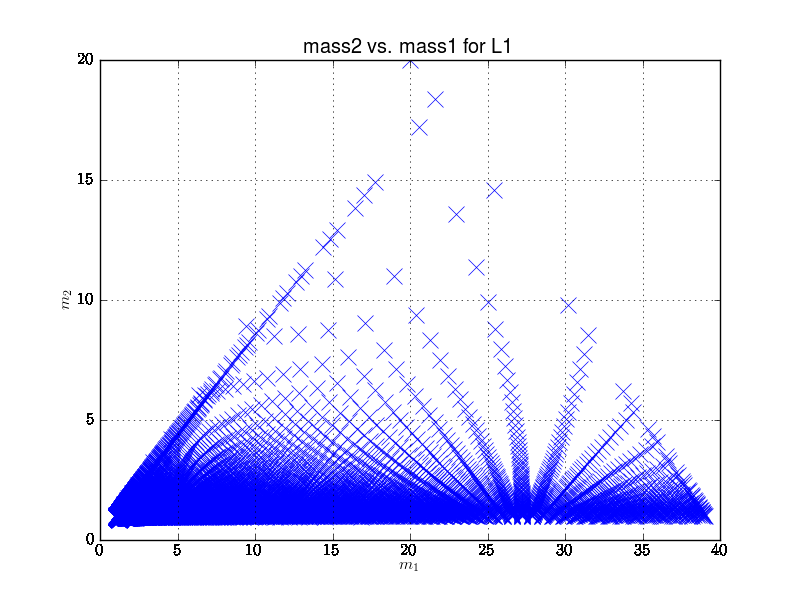
\includegraphics[scale=0.40]{Images/L1_m1m2_tmpltbank_GRB070429B.png}
%\caption{Template bank in $m_2$ vs. $m_1$ -- the $m_2$ is the mass of the larger component.}
%\label{templatebankL1}
\end{minipage}
\hspace{0.5cm}
\begin{minipage}[b]{0.5\linewidth}
%\centering
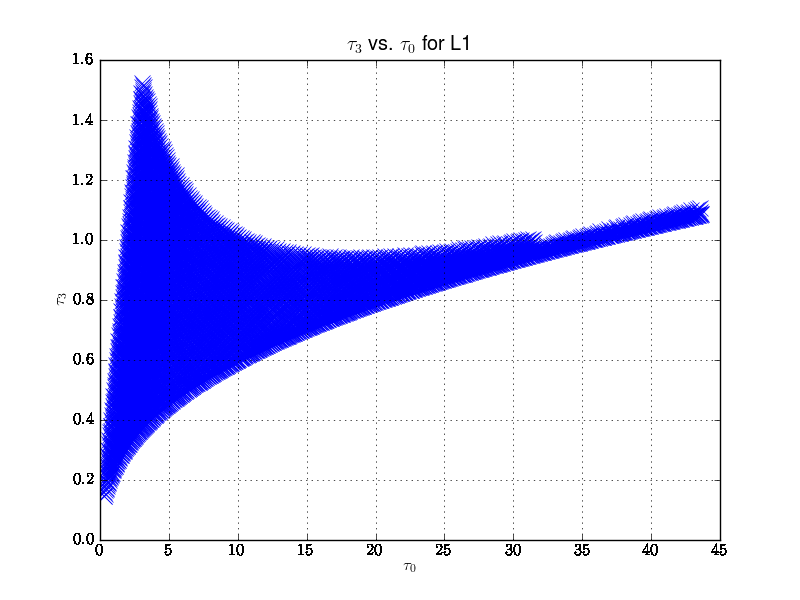
\includegraphics[scale=0.40]{Images/L1_tau0tau3_tmpltbank_GRB070429B.png}
\end{minipage}
\caption{Left figure: template bank in $m_2$ vs. $m_1$ -- the $m_2$ is the mass of the larger component. Right figure: template bank in $\tau_3$ vs. $\tau_0$. The templates are more evenly distributed in $\tau_0$ vs. $\tau_3$ space; this is because the parameter space is approximately flat in $\tau_0$ and $\tau_3$, as discussed .}
\label{tauL1}
%\end{minipage}
\end{figure}

Thus, by using an appropriate set of template waveforms, called a \emph{template bank} in mass space (more precisely in $\tau_0-\tau_3$ space), one can cover all masses in the desired mass interval with some predetermined maximum loss in SNR. Typically, searches will implement a template bank with a maximum SNR loss of 3$\%$, which leads to template banks containing of the order of a few hundred templates (the exact number depends on the detector's noise power spectrum).

\section{The $\chi^2$ test}
\label{chisq_theory}

When noise is Gaussian and stationary the matched filtering technique gives the best probability to find a signal with a before--known waveform. In non--Gaussian data, noise transients (``glitches'') that do \emph{not} match the template but still give high SNR are present. It is necessary to have some way of distinguishing the glitches from true signals.

The method which has become standard for this, is to use a \emph{chi--squared} (${\chi}^2$) veto test \cite{Allen:2004gu}. When a template exceeds a certain threshold SNR, it is then divided into $N$ different frequency bands such that each band should yield $1/N$ of the total SNR of the data if the high SNR event was a signal matching the template. The sum of the squares of the differences between the expected SNR and the actual SNR from each of the $N$ bands is then calculated (the ${\chi}^2$ statistic). The advantage of using the ${\chi}^2$ veto is that glitches tend to produce large ${\chi}^2$ values, and are therefore distinguishable from true gravitational waves signals. Thus, only those template matches with low enough ${\chi}^2$ values are kept for further analysis. We will further detail the theoretical framework of the $\chi^2$ test.

Following the analytic treatment of \cite{Harry:2011qh,ian}, suppose at a given time $t$ the signal in a GW detector will have three components: a Gaussian noise component $n(t)$, a GW signal component that matches a template $h(t)$ and a non--Gaussian component that would match a ``glitch'' template $g(t)$:
%
\begin{equation}
s(t) = n(t) + \alpha h(t) + \beta g(t)
\end{equation}
%
where $\alpha$ and $\beta$ are amplitude terms. $h(t)$ and $g(t)$ are orthogonal and normalized:
%
\begin{equation}
  ( g | g ) = 1 \, , (h | h) = 1 \, ,  ( g | h ) = 0 \, .
\end{equation}
%
In order to construct a $\chi^{2}$ test, we must introduce an additional set of $N$ template waveforms $T^{i}$ to the ones already existing in the template bank. These waveforms are required to be orthonormal and orthogonal to the template bank waveforms denoted by $h$,
%
\begin{equation}
\mathrm{orthogonal ~to}~h(t):  (h|T^i) = 0
\end{equation}
%
\begin{equation}
\mathrm{orthonormality:} ~(T^i | T^j) = \delta^{ij}
\end{equation}
%
The $\chi^{2}$ discriminator is constructed as a sum of squares of the match between $T^i$ and the data stream $s$:
%
\begin{equation}\label{eq:chi2}
  \chi^2 = \sum_{i=1}^{N} (T^i | s)^2 \, .
\end{equation}
%
When the data comprises only signal $h$ and and Gaussian noise $n$, the $\chi^2$ will be
%
\begin{equation}
  \chi^2 = \sum_{i=1}^{N} (T^i | n)^2
\end{equation}
%
and the statistic is the sum of squares of independent Gaussian variables with zero mean and unit variance. Thus the test is $\chi^{2}$ distributed with $N$ degrees of freedom, with a mean and variance of
%
\begin{equation}
  \langle\chi^2\rangle = N
  \quad
  {\rm Var}(\chi^2) = 2N
\end{equation}

In the case where the data is not an exact match to the signal, we take both $\alpha$ and $\beta$ to be non--zero, i.e., any signal or glitch can be linearly decomposed into a part $\alpha h(t)$ and a second orthogonal part $\beta g(t)$. In this case the $\chi^{2}$ test takes the form
%
\begin{equation}
  \chi^2 = \sum_{i=1}^N \left[ (T^i | n)^2 + 2 \beta (T^i | n)(T^i | g) +
  \beta^{2} (T^i|g)^2 \right] \, .  
\end{equation}
%
This has a mean
%
\begin{equation}
  \langle\chi^2\rangle = N + \beta^{2} \sum_i^N (T^i | g)^2
\end{equation}
%
and a variance
%
\begin{equation}
  {\rm Var}(\chi^2) = 2N + 4 \beta^{2} \sum_i^N(T^i|g)^{2} \, .
\end{equation}
%
The $\chi^{2}$ statistic is distributed as a non--central $\chi^{2}$ distribution with $N$ degrees of freedom and a non--centrality parameter \cite{Allen:2004gu}
%
\begin{equation}
  \lambda =  \beta^{2} \sum_{i=1}^N (T^i | g)^2
\end{equation}
%
Let
%
\begin{equation}
 \rho_{\mu}^i =
  \frac{(s | h_{\mu}^i)}{\sqrt{(h_{\mu} | h_{\mu})}}
\end{equation}
%
be the \ac{SNR} contribution in the $i$th frequency bin for the $\mu$th amplitude term. The $\chi^{2}$ statistic is then constructed as
%
\begin{equation}
  \chi^2 = N \sum_{i=1}^N \sum_{\mu = 1}^4 (\rho_{\mu}^i - \rho_{\mu}/N)^2.
\end{equation}
%
As all the components are orthogonal it is easy to see that this statistic will be exactly $\chi^{2}$ distributed with $4(N - 1)$ degrees of freedom. In a coherent way, one can interpret this as the sum of the single detector $\chi^{2}$ values for the $h_{0}$ and $h_{\frac{\pi}{2}}$ waveforms in the synthetic $+$ and $\cross$ detectors. This simply means that the ${\chi}^2$ threshold, ${\chi}^*$, depends quadratically on the measured SNR, ${\rho}$, as well as linearly on the mismatch $\Delta T$ (the threshold represents the maximum value of the $\chi^2$ assigned to signals; it is set fixed for an analysis). The main challenge to constructing a working $\chi^2$ test is the adequate choice of templates $T^i$ to model the effect of glitches in the \ac{GW} data streams \cite{Harry:2011qh,ian}. These are constructed by taking into account three factors: the accuracy of the waveform, the template bank mismatch up to a maximal loss in optimal SNR of 3\%; the uncertainties in instrumental calibration affecting the match between signal and template. Therefore, the coherent analysis will construct three different $\chi^2$ tests to account for these challenges -- we refer the reader to Chapter \ref{Chapter Four}, Section \ref{coh_search_grb}, for an overview of these tests.

\section{Horizon distance}
\label{horizon_distance_theory}

In assessing the overall performance of a detector for CBC searches, we use two representative numbers: the inspiral horizon distance to identify the ``typical'' sensitivity of the interferometers in terms of distance range (which is closely related to the PSD) and the live--time of the detector to identify the amount of time the detector has been on and taking science--mode data during a search (which is closely related to the amount and types of data quality vetoes that are applied to the data, see Chapter \ref{Chapter Four} for reference).  

The inspiral horizon distance of a detector is the distance at which an optimally--oriented and optimally--located equal--mass compact binary inspiral would give an average SNR of $\rho=8$ in the interferometer \cite{Abadie:2010cg}. We find the inspiral horizon distance by setting $\langle \rho \rangle = 8$ in equation (\ref{eq:cbc_fouriermagic}) and solving for the distance $D$ to the inspiral event which parameterizes the waveform $\tilde{h}(f)$.  Thus, the inspiral horizon distance combines the spectral density curve (PSD) with the expected inspiral waveform to produce a single quantity that summarizes the sensitivity of the detector at a given time.

Due to the fact that the detector operates over a frequency range which is not bound at infinity, modifications to the limits of the integral need to be applied.  In the CBC search, we compute the signal to noise ratio by
\begin{eqnarray}
\label{range} \langle \rho \rangle= \sqrt{4 \int_{f_{low}}^{f_{high}} \frac{|\tilde{h}(f)|^2}{S_n(f)} df}.
\end{eqnarray}
The lower limit is determined by the detector's behavior at low frequencies.  In the S5 CBC search the lower frequency cut--off limit was set to $f_{low}=40$ Hz in computing the inspiral horizon distance, since this corresponds to the seismic threshold frequency \cite{Macleod:2011up}.  For Virgo in VSR1, the low frequency cut--off was higher at $f_{low}=60$Hz.  The upper integration bound is the innermost stable circular orbit (ISCO) frequency that separates the inspiral phase to the merger phase (see Chapter \ref{Chapter One} where we have already introduced ISCO)

\begin{eqnarray}
f_{isco} = \frac{c^3}{6\sqrt{6}\pi G M},
\end{eqnarray}
%
where $M$ is the total mass of the binary system.  For binary neutron star systems, $f_{isco}= 1570$Hz.  However, during S5/VSR1 the sampling frequency of the 2048s. blocks used to compute the PSD was $f_{\mathrm{Nyquist}}$ = 2048 Hz. This difference in the upper limit of the frequency has a negligible effect due to the fact that most of the power in SNR is accumulated in the high--sensitivity ``bucket'' of the PSD (see Chapter \ref{Chapter One}, Figure \ref{ligonoise} -- the ``bucket'' is in the region of 100 Hz for LIGO).

For an optimally--oriented and optimally--located equal mass binary, the signal that appears at the interferometer in the approximation of the stationary phase waveform is given by (see Chapter \ref{Chapter One}, equation (\ref{eq:cbc_hp_hc_spa})):

\begin{eqnarray}
\label{spa}
\tilde{h}(f) =  \frac{1}{D}\left(\frac{5\pi }{24c^3}\right)^{1/2}(G\mathcal{M})^{5/6}(\pi f)^{-7/6} e^{i\Psi(f;M)},
\end{eqnarray}

\noindent where $\mathcal{M}$ is the chirp mass of the binary, $D$ is the distance to the binary and $\Psi$ is a real function of $f$, parameterized by the total mass $M$.  Setting $\langle \rho \rangle = 8$ and inserting this waveform into equation (\ref{range}), we find that the inspiral horizon distance is given by:

\begin{eqnarray}
\label{range0} D = \frac{1}{8}\left(\frac{5\pi }{24c^3}\right)^{1/2}(G\mathcal{M})^{5/6}\pi^{-7/6} \sqrt{4 \int_{f_{low}}^{f_{high}} \frac{f^{-7/3}}{S_n(f)}df },
\end{eqnarray}

\noindent where $D$ is expressed in Mpc. The horizon distance is usually calculated for equal mass components. The mean inspiral horizon distance as a function of component mass for the four gravitational wave detectors H1, L1, H2 and V1 during all of S5 and VSR1 science runs is shown in Figure \ref{rangevmass}.

\begin{figure}[ht!]
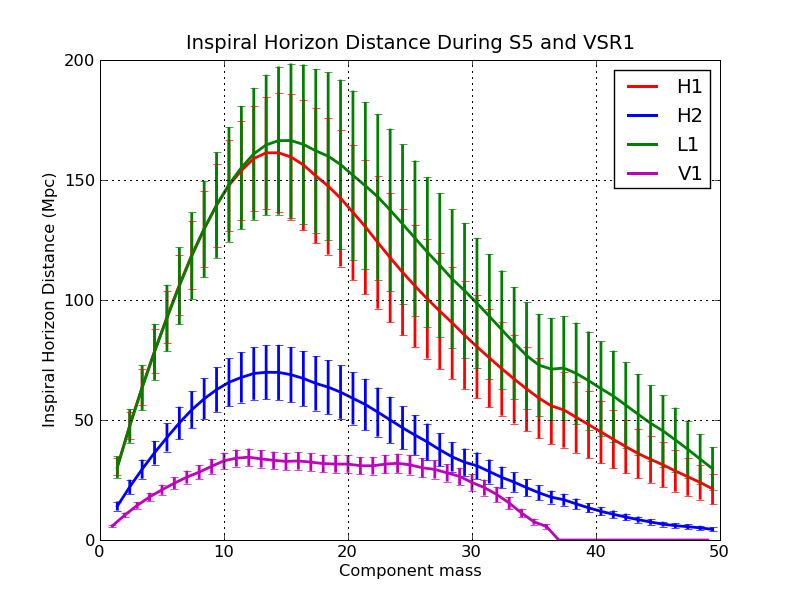
\includegraphics[scale=0.65]{Images/horizon_distance_S5.png}
\caption{Mean inspiral horizon distance as a function of component mass for the four gravitational wave detectors H1, L1, H2 and V1 during all of S5 and VSR1 science runs.  The error bars attached to the points indicate the standard deviation in the inspiral horizon over the course of each of the weeks of the science runs; the error bars extend from one standard deviation below to one standard deviation above the mean. Image first published and reproduced from \cite{Abadie:2010cg}}
\label{rangevmass}
\end{figure}

\newpage
In this chapter we have introduced a series of key theoretical concepts that are used in gravitational waves data analysis. In the next chapter, Chapter \ref{Chapter Four}, we will present the practical use of these concepts in the analysis process with direct application to GW data analysis associated with short GRB triggers.
